
% \begin{figure}[!htp]
%     \centering
%     \begin{subfigure}[b]{0.49\linewidth}
%         \centering
%         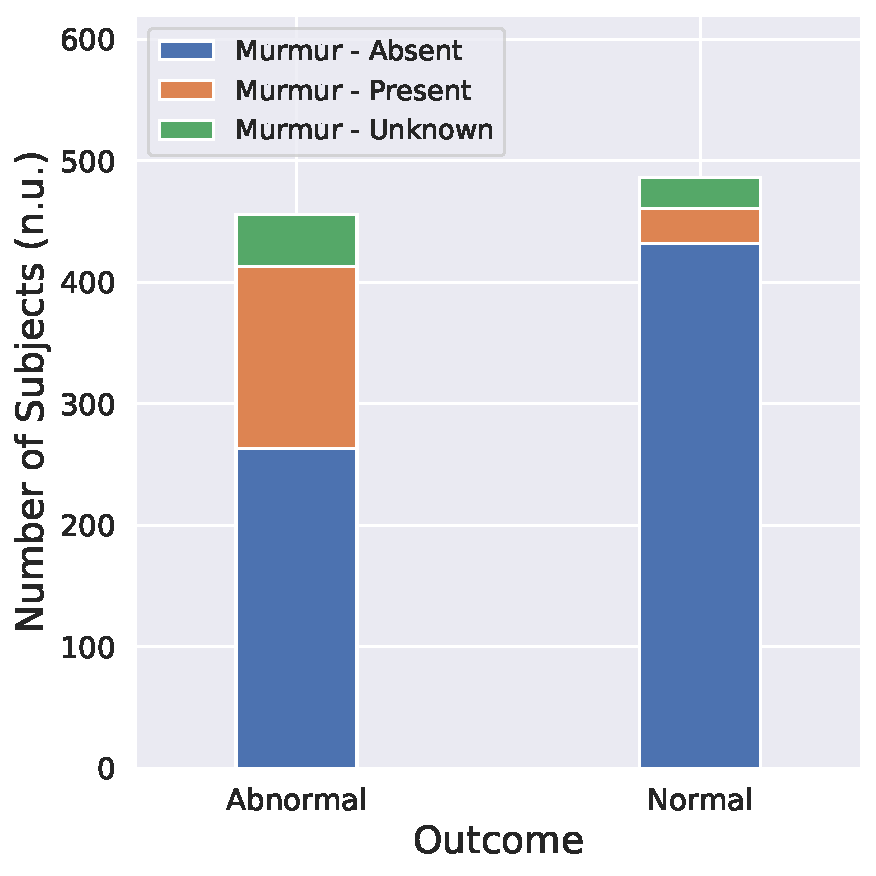
\includegraphics[width=\textwidth]{images/outcome_murmur_corr.pdf}
%         \caption[]
%         {Distribution against the existence of heart murmurs.}
%         \label{fig:outcome_murmur_corr}
%     \end{subfigure}
%     \hfill
%     \begin{subfigure}[b]{0.49\linewidth}
%         \centering
%         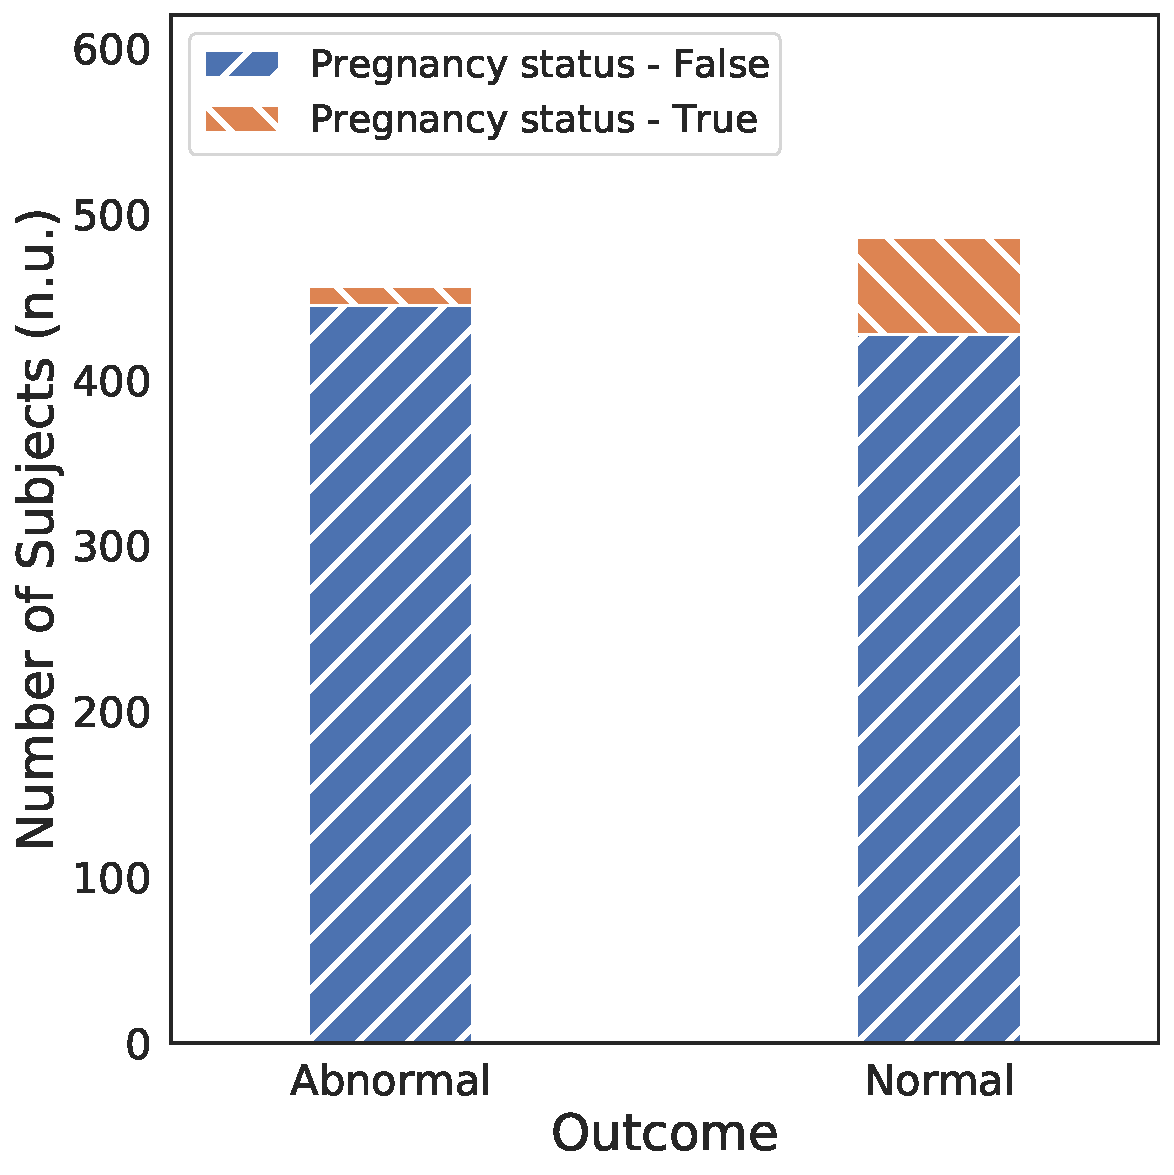
\includegraphics[width=\textwidth]{images/outcome_pregnancy_status_corr.pdf}
%         \caption[]
%         {Distribution against pregnancy status.}
%         \label{fig:outcome_pregnancy_status_corr}
%     \end{subfigure}
%     \vskip\baselineskip
%     \begin{subfigure}[b]{0.49\linewidth}
%         \centering
%         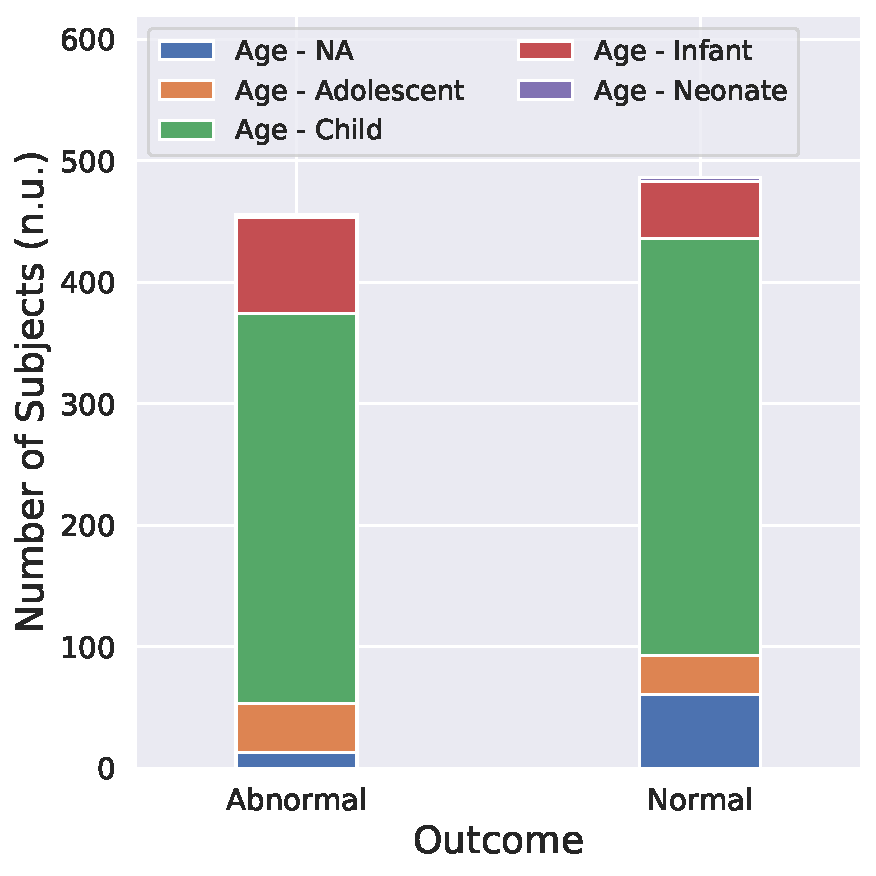
\includegraphics[width=\textwidth]{images/outcome_age_corr.pdf}
%         \caption[]
%         {Distribution against age.}
%         \label{fig:outcome_age_corr}
%     \end{subfigure}
%     \hfill
%     \begin{subfigure}[b]{0.49\linewidth}
%         \centering
%         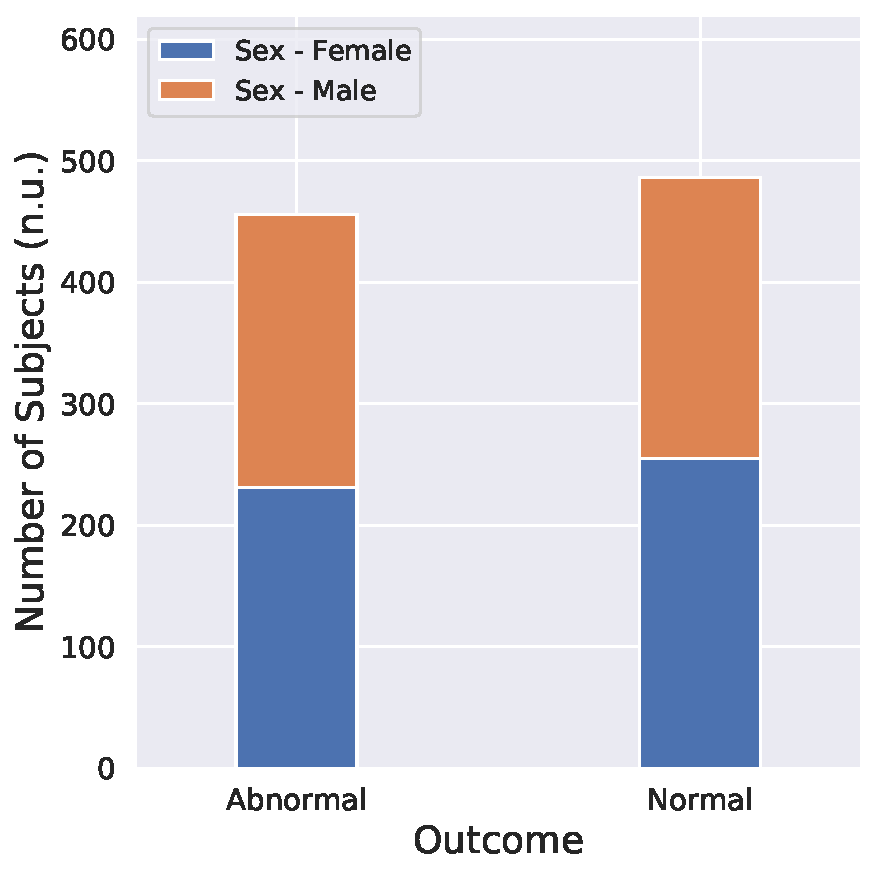
\includegraphics[width=\textwidth]{images/outcome_sex_corr.pdf}
%         \caption[]
%         {Distribution against sex.}
%         \label{fig:outcome_sex_corr}
%     \end{subfigure}
%     \caption[]
%     {Distribution of outcome against 4 typical categorical demographic variables.}
%     \label{fig:outcome_corr}
%     \end{figure}



\begin{figure}[!htp]
\centering
\begin{subfigure}[t]{0.49\linewidth}
    \centering
    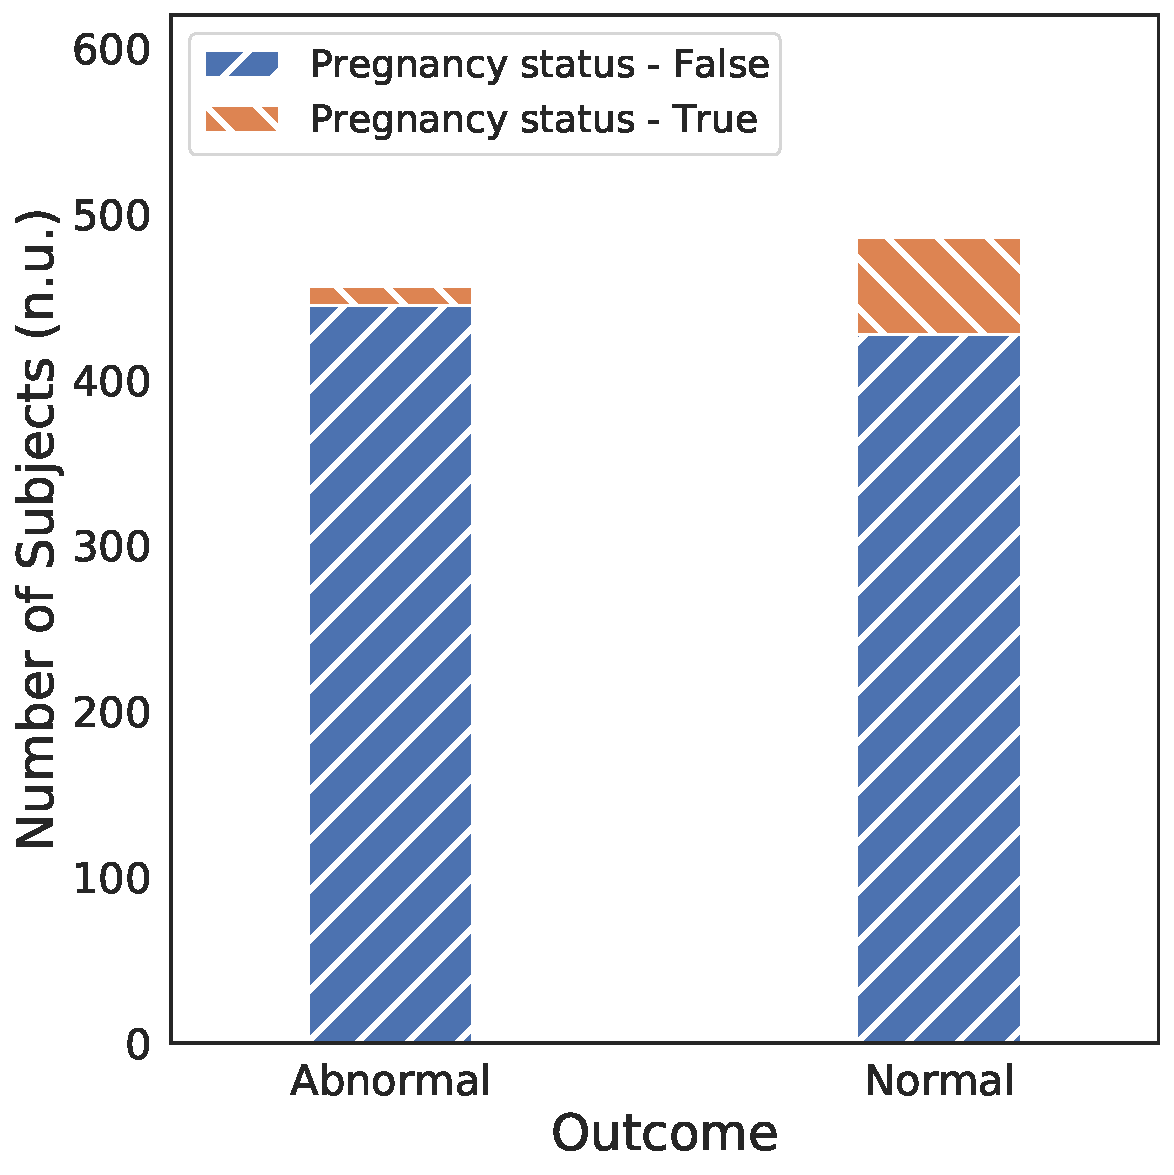
\includegraphics[width=\textwidth]{images/outcome_pregnancy_status_corr.pdf}
    \caption[]
    {Distribution against pregnancy status.}
    \label{fig:outcome_pregnancy_status_corr}
\end{subfigure}
\hfill
\begin{subfigure}[t]{0.49\linewidth}
    \centering
    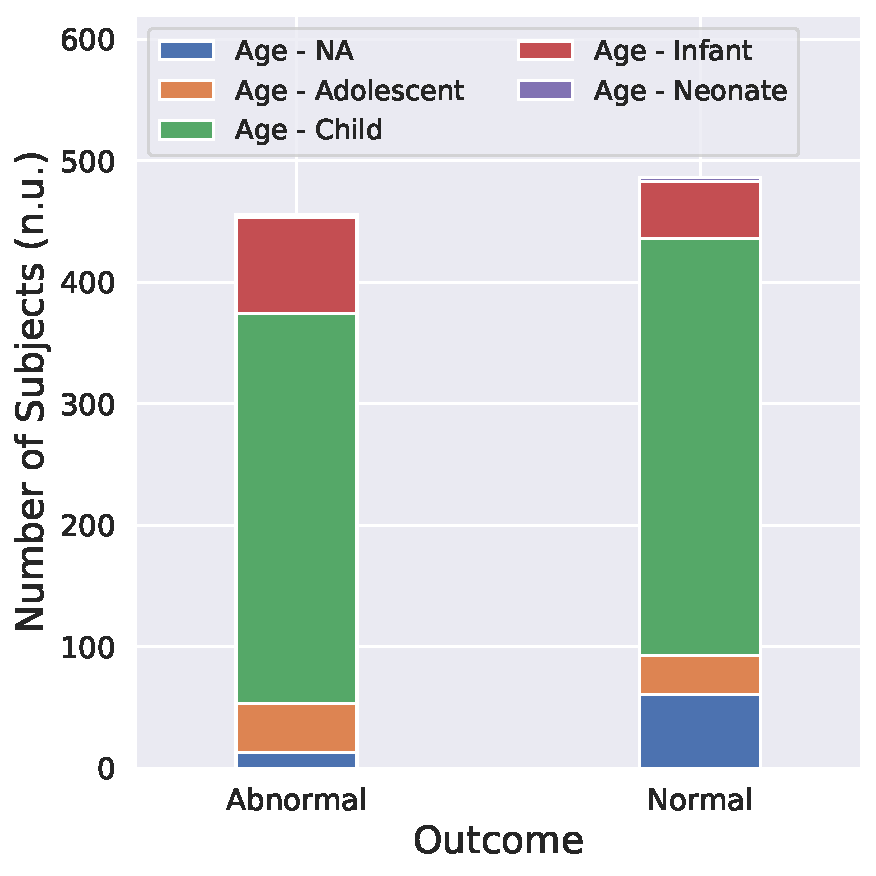
\includegraphics[width=\textwidth]{images/outcome_age_corr.pdf}
    \caption[]
    {Distribution against age.}
    \label{fig:outcome_age_corr}
\end{subfigure}
\caption[]
{Distributions of the ``Outcome'' against 2 typical categorical demographic variables.}
\label{fig:outcome_corr}
\end{figure}
